\documentclass[11pt,a4paper,english]{paper}
\usepackage{mathtools}
\usepackage[breakable]{tcolorbox}
%\usepackage{minted}
\newtcolorbox{mybox}[1]{colback=red!5!white,colframe=red!75!black,fonttitle=\bfseries,title=#1,breakable}
\newtcolorbox{bluebox}[1]{colback=blue!5!white,colframe=blue!75!black,fonttitle=\bfseries,title=#1,breakable}
\newtcolorbox{gbox}[1]{colback=green!5!white,colframe=green!75!black,fonttitle=\bfseries,title=#1,breakable}
\newtcolorbox{bbox}[1]{colback=black!5!white,colframe=black!75!black,fonttitle=\bfseries,title=#1,breakable}
\usepackage{amsmath}                                    % extensive math options
\usepackage{amssymb}                                    % special math symbols
\usepackage[mathlines]{lineno}
\usepackage[Gray,squaren,thinqspace,thinspace]{SIunits} % elegant units
\usepackage{listings}                                   % source code

\usepackage{graphicx}
\graphicspath{ {./} }
%\setminted{breaklines}

\begin{document}

\title{CS 008 \\ Lecture notes \\ 3/19/24}
\maketitle

\section{Outline}

\begin{itemize} {

    \item Announcements

    \item Template classes

    \item Data structures \& algorithms

      \begin{itemize} {

          \item Big-O notation
          \item Stacks
          \item Queue

      }\end{itemize}

}\end{itemize}

\section{Announcements}

\begin{gbox}{Exam:} {
  Exam is next Thursday (3/28/24)
  }
\end{gbox}


\section{Template classes}

As the name implies, the idea of a \textbf{template} class unlike a regular class would be the ability to pass in the data type as a parameter so that there is no need to create the same class for different parameters.
\newpage

\section{Big-O notation review}

Consider a function: $f(n) = a_{j}n^{j} + a_{j-1}n^{j-1} + ... + a_{1}n + a_0$, what would be the complexity time of this function? (If all variables of a are constants)



\bigskip

\noindent Looking at the function, you only consider the \textbf{largest} term in the function (which would be $a_{j}n^j$) and then drop the constant resulting in a time complexity of $O(n^{j})$.

\bigskip

\noindent Now, consider the same function but with a small change: $f(n) = a_{j}n^{j} + a_{j-1}n^{j-1} + ... + a_{1}n + a_0 + b\log(n)$. The complexity class of the function given is still $O(n^{j})$ since the largest term has not changed. However, if $b$ is a constant of $10^{20}!$ (a very large number), what would happen to the complexity time?

\[ \textbf{It will still be $O(n^{j})$.}\]

\bigskip

\begin{gbox}{Question:} {

    If we added $c * 2^{n}$ to the end of the function, would the time complexity change?

    \bigskip

    \textbf{Answer}: Yes, at a large enough value for $n$, the value of $c * 2^{n}$ would exceed the largest term in the original function.


}\end{gbox}

\bigskip

\noindent Big-O classes represent \textit{upper bounds} on runtime.

\bigskip

\begin{bbox}{Figure 1:} {


        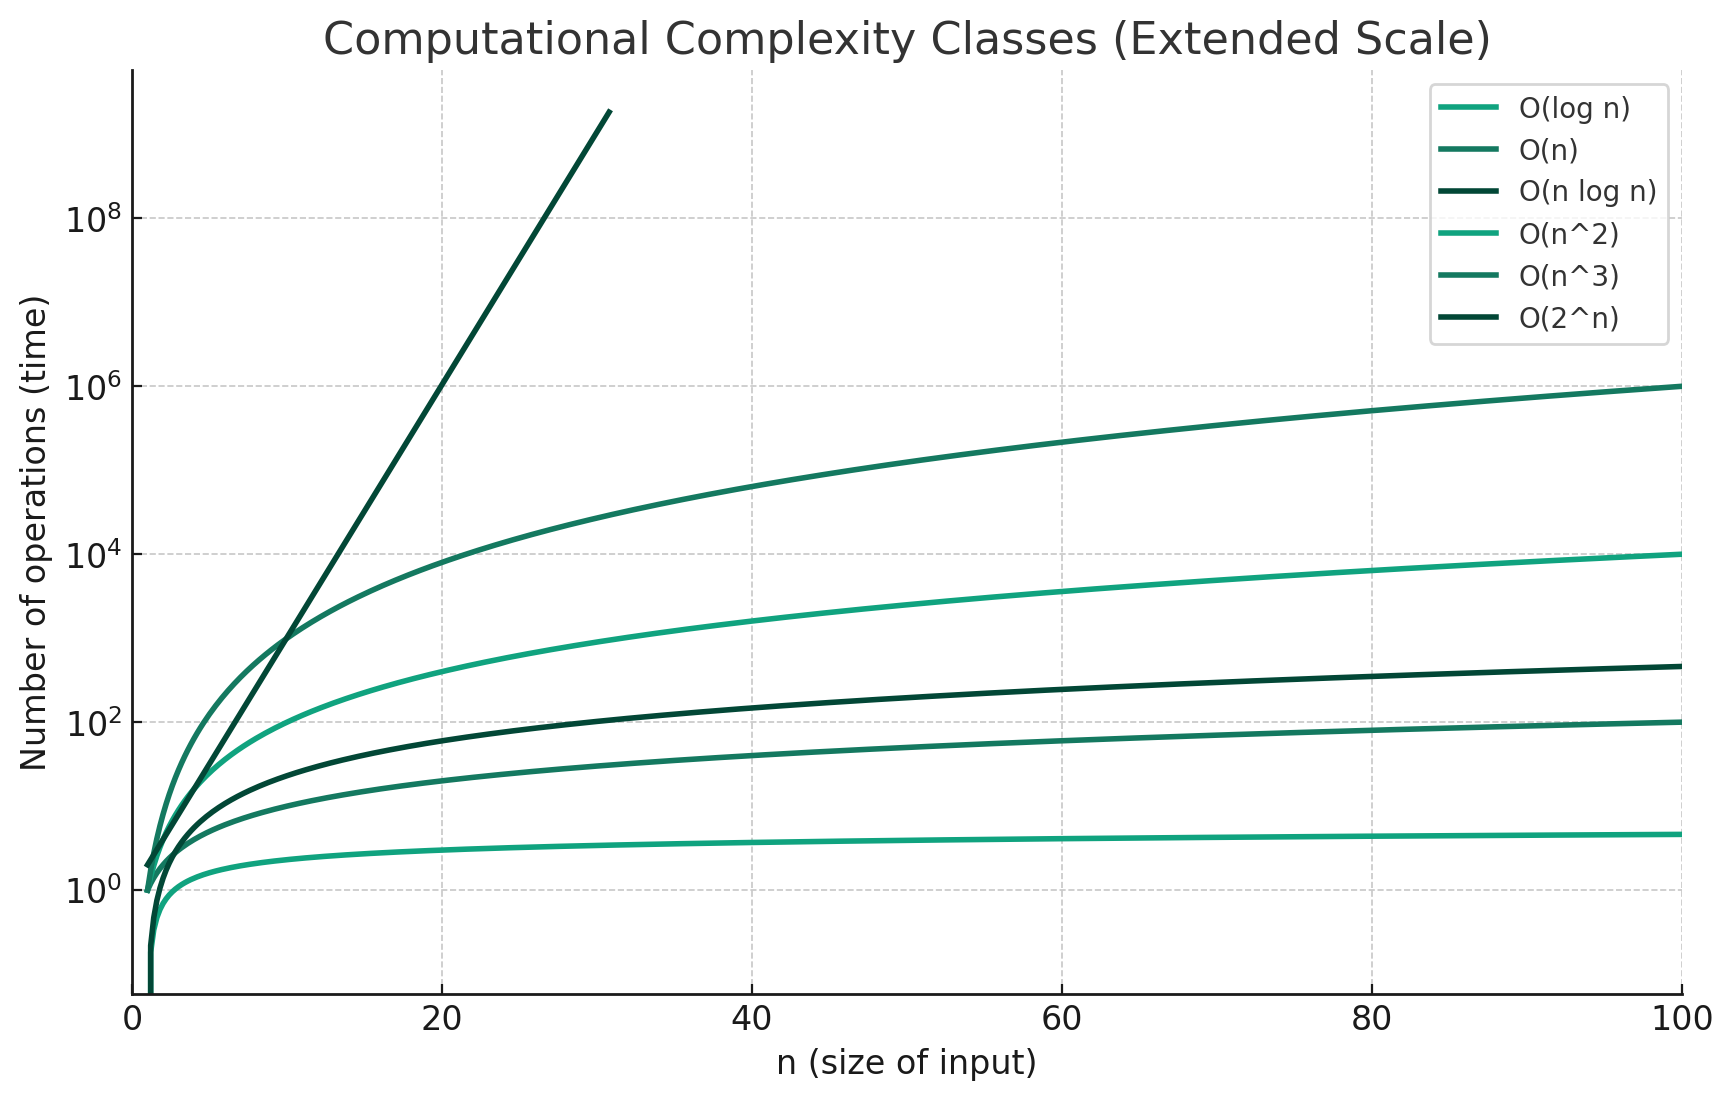
\includegraphics[width=\textwidth]{o_vs_n.png}
}\end{bbox}

\bigskip

\begin{bluebox}{Note:} {

Sometimes, you might encounter something like $f(n) = O(n)$ however, a better way to describe a function that has a certain time complexity would be: $f(n) \in O(n)$.

  }
\end{bluebox}

\bigskip

\begin{bluebox}{Definition:} {

    If $f(n) \in O(n^{k})$, then there exists an integer $N$ and a real number $G$ which depends on $N$ such that for all values of $n \geq N$: $f(n) \leq G*n^{k}$.

}\end{bluebox}

\bigskip

\section{Stacks}

A \textbf{stack} is an abstract data type and is a 1-dimensional container class containing many objects of one certain type which can only add and remove from one end and is known as \textbf{LIFO} (\textit{last in, first out}). Consider a stack of books, intuitively we know that a stack of books would need to be removed from the top to bottom. New books would be added to the top and will also be the first ones to be removed.

\newpage
\noindent A \textbf{stack} contains a few important functions:
\begin{itemize} {
    \item pop(): remove top item
    \item push(): add item to top
    \item top(): view top item
    \item empty(): check if stack is empty
    \item size(): check the size of the stack
}\end{itemize}

\bigskip

\begin{gbox}{Question:} {

  What's the difference between an \textbf{abstract data type} and a \textbf{data structure}?

  \bigskip
  \textbf{Answer}: A data structure is an implementation of an abstract data type.

}\end{gbox}


\bigskip
\begin{bluebox}{Note:} {
C++ has a built-in stack ( include stack ) that already exists. 
*insert example code*
} \end{bluebox}

\bigskip
\noindent Possible implementations of a stack:
\begin{itemize} {

  \item static-length array
  \item dynamic array
  \item linked-list

}\end{itemize}

\end{document}

